%==================================================================
%  DEFENSA DE TESIS DOCTORAL  -  Rubén D. Ledesma
%  "Mejora de la representatividad espacial de estimaciones de
%   radiación solar de bases de datos satelitales, para Salta y
%   Jujuy, usando herramientas de Inteligencia Artificial."
%
%  Compilar con pdflatex (2 pasadas).
%  Las figuras se buscan en ./figuras/ (igual que en la tesis).
%  Si una figura no está, se muestra un marcador y NO rompe nada.
%==================================================================
\documentclass[aspectratio=169,11pt]{beamer}

\usepackage[utf8]{inputenc}
\usepackage[T1]{fontenc}
\usepackage[provide=*,spanish]{babel}
\usepackage{amsmath,amssymb}
\usepackage{booktabs}
\usepackage{tikz}
\usepackage{pgfplots}
\pgfplotsset{compat=1.18}
\usetikzlibrary{positioning,arrows.meta,calc,shapes.geometric}
\usepackage{graphicx}
\graphicspath{{figuras/}{./}}

%------------------------------------------------------------------
%  PALETA Y TEMA (look propio, sin dependencias de fuentes externas)
%------------------------------------------------------------------
\definecolor{primary}{HTML}{1F3A5F}   % azul profundo
\definecolor{accent}{HTML}{E59500}    % ámbar solar
\definecolor{teal}{HTML}{2A7F8E}      % verde azulado
\definecolor{lightbg}{HTML}{F4F6F9}
\definecolor{darktext}{HTML}{1A1A1A}
\definecolor{midgray}{HTML}{6B7280}

\usetheme{default}
\usecolortheme{default}
\setbeamertemplate{navigation symbols}{}
\setbeamercolor{normal text}{fg=darktext}
\setbeamercolor{structure}{fg=primary}
\setbeamercolor{frametitle}{fg=white,bg=primary}
\setbeamercolor{title}{fg=primary}
\setbeamercolor{item}{fg=accent}
\setbeamercolor{block title}{fg=white,bg=teal}
\setbeamercolor{block body}{bg=lightbg,fg=darktext}
\setbeamercolor{alerted text}{fg=accent}
\setbeamerfont{frametitle}{series=\bfseries,size=\large}
\setbeamerfont{title}{series=\bfseries}
\setbeamertemplate{itemize item}{\color{accent}\textbullet}
\setbeamertemplate{itemize subitem}{\color{teal}--}

% Título de frame con regla ámbar inferior
\setbeamertemplate{frametitle}{%
  \nointerlineskip
  \begin{beamercolorbox}[wd=\paperwidth,ht=2.4em,dp=0.6em,leftskip=0.5cm,rightskip=0.5cm]{frametitle}%
    \vbox to 1.6em{\vfil\strut\insertframetitle\vfil}%
  \end{beamercolorbox}%
  {\color{accent}\rule{\paperwidth}{1.6pt}}%
}

% Pie de página minimalista
\setbeamertemplate{footline}{%
  \hbox{%
    \begin{beamercolorbox}[wd=.62\paperwidth,ht=2.3ex,dp=1ex,leftskip=0.4cm]{}%
      \tiny\color{midgray} R. D. Ledesma — Defensa doctoral%
    \end{beamercolorbox}%
    \begin{beamercolorbox}[wd=.38\paperwidth,ht=2.3ex,dp=1ex,rightskip=0.4cm]{}%
      \hfill\tiny\color{midgray}\insertframenumber/\inserttotalframenumber%
    \end{beamercolorbox}}%
}

%------------------------------------------------------------------
%  MACRO DE FIGURA CON FALLBACK (no rompe si falta el archivo)
%------------------------------------------------------------------
\newcommand{\phbox}[1]{%
  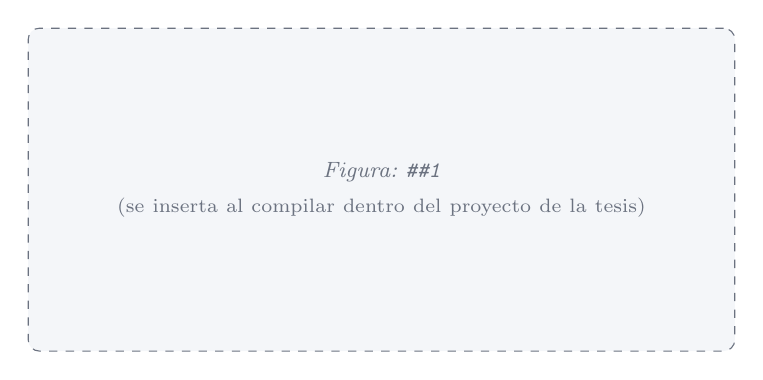
\begin{tikzpicture}
    \node[draw=midgray,dashed,fill=lightbg,rounded corners,
          minimum width=0.74\linewidth,minimum height=4.1cm,
          align=center,text=midgray,font=\footnotesize\itshape,
          text width=0.66\linewidth]
      {Figura: \texttt{\detokenize{#1}}\\[3pt]\normalfont\scriptsize(se inserta al compilar dentro del proyecto de la tesis)};
  \end{tikzpicture}}

% \sfig[ancho]{archivo}  -> intenta figuras/archivo, luego archivo, luego placeholder
\newcommand{\sfig}[2][\linewidth]{%
  \IfFileExists{figuras/#2}{\includegraphics[width=#1]{figuras/#2}}{%
    \IfFileExists{#2}{\includegraphics[width=#1]{#2}}{\phbox{#2}}}}

% Bloque de "mensaje clave"
\newcommand{\clave}[1]{%
  \begin{beamercolorbox}[wd=\linewidth,sep=6pt,rounded=true]{block body}%
    \footnotesize\textbf{\color{primary}Idea clave: }#1%
  \end{beamercolorbox}}

%------------------------------------------------------------------
%  PORTADA DE SECCIÓN
%------------------------------------------------------------------
\AtBeginSection[]{%
  \begin{frame}[plain]
    \begin{tikzpicture}[remember picture,overlay]
      \fill[primary] (current page.south west) rectangle (current page.north east);
      \fill[accent] ([yshift=-0.9cm]current page.west) rectangle ([yshift=-1.05cm]current page.east);
    \end{tikzpicture}
    \vfill
    \centering
    {\color{white}\small\bfseries Parte \insertsectionnumber}\\[0.5em]
    {\color{white}\Large\bfseries\insertsection}
    \vfill
  \end{frame}}

%------------------------------------------------------------------
\title{Mejora de la representatividad espacial de estimaciones de radiación solar de bases de datos satelitales para Salta y Jujuy mediante Inteligencia Artificial}
\author{Rubén D. Ledesma}
\date{\today}

%==================================================================
\begin{document}

%------------------ PORTADA ------------------
\begin{frame}[plain]
  \begin{tikzpicture}[remember picture,overlay]
    \fill[primary] (current page.north west) rectangle ([yshift=-1.9cm]current page.north east);
    \fill[accent] ([yshift=-1.9cm]current page.north west) rectangle ([yshift=-2.05cm]current page.north east);
  \end{tikzpicture}
  \vspace{1.1cm}
  {\color{white}\hfill\footnotesize Tesis Doctoral\hspace{0.6cm}}

  \vspace{1.6cm}
  {\color{primary}\bfseries\large Mejora de la representatividad espacial de\\[2pt] estimaciones de radiación solar de 
  Bases de Datos Satelitales\\[2pt]
   para Salta y Jujuy, usando herramientas de Inteligencia Artificial}


  \vspace{0.5em}
  {\color{accent}\rule{0.55\linewidth}{1.4pt}}

  \vspace{0.8em}
  {\bfseries Lic. Rubén D. Ledesma}\\[0.3em]
  {\footnotesize\color{midgray} Universidad Nacional de Salta}

  \vfill
  {\scriptsize\color{midgray}
   Director: Dr. Germán Salazar \quad\textbar\quad %Co-director/a: [completar]\\[2pt]
   Jurado: Dr. Rodrigo Alonso-Suárez, Dr. Raúl Righini, Dr. Javier Trenti\\[2pt] \hfill 6 de Julio de 2026}
  \vspace{0.4cm}
\end{frame}

%------------------ HOJA DE RUTA ------------------
\begin{frame}{Estructura de la presentación}
  \footnotesize
  \begin{columns}[T]
    \column{0.5\linewidth}
    \begin{enumerate}
      \item Motivación y problema
      \item Marco: Adaptación al Sitio + Aprendizaje Automático
      \item Datos y zona de estudio (NOA)
      \item Diagnóstico: modelos sin adaptar
    \end{enumerate}
    \column{0.5\linewidth}
    \begin{enumerate}\setcounter{enumi}{4}
      \item Resultados: cuatro enfoques de adaptación
      \item Generalización espacial
      \item Conclusiones y perspectivas
    \end{enumerate}
  \end{columns}
  \vspace{0.6em}
  \clave{Una hipótesis central — \emph{integrar Aprendizaje Automático permite capturar relaciones no lineales entre la irradiancia modelada y variables locales, reduciendo el error de las estimaciones y extendiendo la corrección a celdas sin medición.}}
\end{frame}

%==================================================================
\section{Motivación y problema}
%==================================================================

\begin{frame}{El recurso solar es estratégico... y hay que medirlo bien}
  \footnotesize
  \begin{columns}[T]
    \column{0.56\linewidth}
    \begin{itemize}
      \item En 2024 la generación fotovoltaica superó los \textbf{2.000 TWh} ($\approx 7\%$ de la electricidad mundial).
      \item Diseñar, financiar y operar plantas FV exige conocer el recurso solar (GHI) con precisión, en el espacio y en el tiempo.
      \item La GHI es además una variable transversal: clima, hidrología, agricultura, ambiente.
    \end{itemize}
    \vspace{0.3em}
    \clave{Sin una buena caracterización del recurso, todo lo que se construye encima (energía, financiamiento, clima) hereda el error.}
    \column{0.44\linewidth}
    \centering
    \sfig[\linewidth]{sites.png}\\
    {\scriptsize\color{midgray} Noroeste Argentino (NOA): alto potencial solar, baja densidad de medición.}
  \end{columns}
\end{frame}

\begin{frame}{El problema en dos planos: espacial y temporal}
  \footnotesize
  \begin{columns}[T]
    \column{0.5\linewidth}
    \textbf{\color{primary}Medir en superficie es lo más fiable...}
    \begin{itemize}
      \item Piranómetros homologados (ISO 9060:2018), dataloggers, calibración y mantenimiento.
      \item Caro y logísticamente difícil de sostener.
    \end{itemize}
    \textbf{\color{primary}...pero es escaso e intermitente}
    \begin{itemize}
      \item \emph{Problema espacial}: no se puede medir en todos los sitios necesarios.
      \item \emph{Problema temporal}: registros con \emph{gaps}, series cortas.
    \end{itemize}
    \column{0.5\linewidth}
    \begin{block}{Contexto argentino}
      \scriptsize
      \begin{itemize}
        \item \textbf{Sin estaciones BSRN} en el país.
        \item Proyecto ENARSOL (2012, 40 estaciones) discontinuado.
        \item El NOA: alto potencial, muy baja densidad radiométrica y sin trazabilidad sistemática.
      \end{itemize}
    \end{block}
  \end{columns}
\end{frame}

\begin{frame}{La alternativa: satélite y reanálisis — cobertura, pero con error}
  \footnotesize
  \begin{columns}[T]
    \column{0.52\linewidth}
    \textbf{\color{teal}Resuelven la cobertura}
    \begin{itemize}
      \item Satélite (desde 1997) y reanálisis (desde 1940): regiones enteras, series largas y continuas.
    \end{itemize}
    \textbf{\color{accent}Pero son estimaciones de un modelo}
    \begin{itemize}
      \item No son mediciones: arrastran sesgos sistemáticos y errores.
      \item El error se agrava en \textbf{topografía compleja} (Salta y Jujuy): nubosidad y efectos orográficos mal representados.
    \end{itemize}
    \column{0.48\linewidth}
    \begin{block}{Por qué importa el error}
      \scriptsize
      Sobreestimar la GHI un 10\% sobreestima la energía generada (MWh/año) y los ingresos $\Rightarrow$ riesgo en la bancabilidad de un proyecto FV.\\[3pt]
      En generación domiciliaria, esperar $5{,}5$ y obtener $4{,}8$ kWh/m²/día desalienta al usuario.
    \end{block}
    \vspace{0.2em}
    \clave{El error de la estimación se \emph{propaga} a todo lo que la usa como entrada.}
  \end{columns}
\end{frame}

\begin{frame}{Pregunta, hipótesis y objetivo}
  \footnotesize
  \begin{block}{Pregunta}
    ¿Cómo corregir las estimaciones satelitales/reanálisis usando las pocas mediciones disponibles, y \emph{propagar} esa corrección a zonas sin medición en Salta y Jujuy?
  \end{block}
  \begin{block}{Hipótesis}
    El aprendizaje automático permite capturar relaciones \textbf{no lineales} entre la irradiancia modelada y las variables locales, reduciendo errores y sesgos sistemáticos de las bases satelitales.
  \end{block}
  \begin{block}{Objetivo}
    Desarrollar, adaptar y evaluar modelos que mejoren la precisión y la representatividad espacial de la GHI en el NOA, y proponer estrategias para extender las correcciones a celdas sin medición directa.
  \end{block}
\end{frame}

%==================================================================
\section{Adaptación al Sitio y Aprendizaje Automático}
%==================================================================

\begin{frame}{¿Qué es la Adaptación al Sitio (SA)?}
  \footnotesize
  \textbf{Definición operativa.} Conjunto de métodos estadísticos que corrigen errores sistemáticos y aleatorios de las estimaciones modeladas, usando \textbf{mediciones de superficie} de un período corto como referencia.
  \vspace{0.4em}
  \begin{block}{Analogía del termómetro}
    \scriptsize
    Un agricultor escucha el pronóstico (la \emph{estimación}). Instala un termómetro y mide un tiempo (la \emph{medición local}). Descubre un sesgo fijo (\,$-5\,$°C en invierno, $+3\,$°C en verano) y lo corrige. Aun cuando retira el sensor, las estimaciones corregidas representan mejor su finca. \textbf{Eso es SA.}
  \end{block}
  \clave{Un período breve de medición de calidad alcanza para corregir series largas — bajo el supuesto de que la relación se mantiene estable.}
\end{frame}

\begin{frame}{Proceso conceptual: ajustar en el solapamiento, aplicar a toda la serie}
  \footnotesize
  \begin{columns}[T]
    \column{0.46\linewidth}
    \textbf{Dos pasos}
    \begin{enumerate}
      \item \textbf{Ajuste}: en el período de \emph{overlap} (medición $\cap$ estimación) se entrena la función de corrección.
      \item \textbf{Aplicación}: la función se extiende a toda la serie modelada.
    \end{enumerate}
    \vspace{0.3em}
    En su forma más simple:
    \[ \mathrm{GHI}_{\text{adaptada}} = f(\mathrm{GHI}_{\text{modelada}}) \]
    \column{0.54\linewidth}
    \centering
    \sfig[\linewidth]{scatter-01.png}\\
    {\scriptsize\color{midgray} Antes (rojo): sesgo bajo la línea 1:1. Después (verde): alineado a 1:1.}
  \end{columns}
\end{frame}

\begin{frame}{Estado del arte: de lo estadístico a lo no lineal}
  \footnotesize
  \textbf{Cinco familias de SA} (Polo et al., 2016 — IEA Task 46): físicos · estadísticos · híbridos · post-proceso · combinados.
  \vspace{0.3em}
  \begin{block}{El giro hacia Machine Learning}
    \scriptsize
    \begin{itemize}
      \item \textbf{Babar (2020)}: Random Forest sobre CLARA-A2/ERA5; corrige el sesgo y reduce el RMSE — de los primeros en usar ML para la función de ajuste.
      \item \textbf{Narváez (2021)}: RF $\approx 38\%$ mejor que QM/MLR en series horarias.
      \item \textbf{Salamalikis (2022)}: modela $\Delta_{\mathrm{GHI}} = \mathrm{GHI}_{med}-\mathrm{GHI}_{mod}$ (desestacionaliza); sesgo $-50\%$.
      \item \textbf{Zainali (2024)}: ML supera a lo estadístico, pero el resultado depende del régimen climático.
    \end{itemize}
  \end{block}
  \clave{La literatura ya advierte: \emph{no existe un modelo universalmente superior}; el resultado depende del sitio.}
\end{frame}

\begin{frame}{Características, ventajas y límites de la SA}
  \scriptsize
  \begin{columns}[T]
    \column{0.5\linewidth}
    \textbf{\color{teal}Ventajas}
    \begin{itemize}
      \item Reducción significativa del sesgo.
      \item Mejora consistente de las métricas.
      \item Flexibilidad: de modelos simples a ML.
    \end{itemize}
    \textbf{\color{primary}Características}
    \begin{itemize}
      \item $\sim 1$ año de overlap suele bastar para entrenar.
      \item Aplicable a satélite y reanálisis, en varias escalas.
    \end{itemize}
    \column{0.5\linewidth}
    \textbf{\color{accent}Límites}
    \begin{itemize}
      \item Requiere datos locales de alta calidad.
      \item Alcance esencialmente \textbf{local}.
      \item No todos los métodos generalizan entre regiones.
      \item \textbf{Estacionariedad temporal}: el ajuste se calibra en un overlap corto y se extrapola a décadas — supone que la relación no deriva (degradación de sensores, cambio de plataforma, deriva de aerosoles).
    \end{itemize}
  \end{columns}
  \vspace{0.3em}
  \clave{El supuesto de estacionariedad es el flanco honesto del método y reaparece al final de esta defensa.}
\end{frame}

\begin{frame}{Modelos de regresión empleados}
  \footnotesize
  \begin{columns}[T]
    \column{0.5\linewidth}
    \textbf{Lineales}
    \begin{itemize}
      \item \textbf{SLR}: un regresor ($\mathrm{GHI}_{mod}$).
      \item \textbf{MLR}: varios regresores; interpretable, barato.
    \end{itemize}
    \textbf{No lineales}
    \begin{itemize}
      \item \textbf{MLP} (perceptrón multicapa): aproximador universal; riesgo de sobreajuste.
      \item \textbf{Random Forest / XGBoost}: ensambles de árboles; capturan no linealidades e interacciones.
    \end{itemize}
    \column{0.5\linewidth}
    \centering
    %\sfig[0.92\linewidth]{MLP.png}\\
    %{\scriptsize\color{midgray} Esquema de un MLP.}
  \end{columns}
  \vspace{0.2em}
  \clave{En SA, $\mathrm{GHI}_{mod}$ \emph{debe} estar entre los regresores: si no, deja de ser adaptación y pasa a ser estimación.}
\end{frame}

\begin{frame}{Entrenamiento, validación, prueba y métricas}
  \footnotesize
  \begin{columns}[T]
    \column{0.52\linewidth}
    \textbf{Partición} (siguiendo Polo 2016/2020, $\geq 1$ año de calibración)
    \begin{itemize}
      \item Entrenamiento / validación / prueba independientes.
      \item Control del sobreajuste y búsqueda de hiperparámetros.
    \end{itemize}
    \column{0.48\linewidth}
    \textbf{Métricas} (relativas, \% de la media medida)
    \begin{align*}
      \mathrm{MBE} &= \tfrac{1}{n}\textstyle\sum (y_i-x_i)\\
      \mathrm{MAE} &= \tfrac{1}{n}\textstyle\sum |y_i-x_i|\\
      \mathrm{RMSE}&= \sqrt{\tfrac{1}{n}\textstyle\sum (y_i-x_i)^2}
    \end{align*}
  \end{columns}
  \vspace{0.2em}
  {\scriptsize $x$: medido, $y$: estimado. \textbf{MBE}=sesgo; \textbf{MAE/RMSE}=dispersión (RMSE penaliza outliers).}
  \clave{Todo se reporta en \% relativo a la media de GHI de cada sitio: hace comparables valle y altiplano.}
\end{frame}

%==================================================================
\section{Datos y zona de estudio}
%==================================================================

\begin{frame}{Cinco estaciones del NOA}
  \scriptsize
  \begin{columns}[T]
    \column{0.46\linewidth}
    \centering
    \sfig[\linewidth]{sites.png}
    \column{0.54\linewidth}
    \renewcommand{\arraystretch}{1.15}
    \begin{tabular}{@{}llccl@{}}
      \toprule
      \textbf{ID} & \textbf{Sitio} & \textbf{Período} & \textbf{Alt. (m)} & \textbf{Clima}\\
      \midrule
      Yu  & Yuto       & 2017--2018 & 401  & Cwa\\
      Sa  & Salta      & 2009--2020 & 1233 & Cwb\\
      Sca & San Carlos & 2012--2013 & 1624 & Cwb\\
      Ero & El Rosal   & 2016--2018 & 3355 & BSk\\
      Lq  & La Quiaca  & 2018--2023 & 3500 & BSk\\
      \bottomrule
    \end{tabular}
    \vspace{0.5em}
    \begin{itemize}
      \item Amplio rango altitudinal y climático.
      \item GHI a 1 minuto (promedio de 6 muestras a 10 s).
      \item Köppen–Geiger; piranómetros ISO 9060:2018 clase A/B.
    \end{itemize}
  \end{columns}
\end{frame}
 

\begin{frame}{Heterogeneidad instrumental: un piso de error desigual}
  \scriptsize
  \begin{columns}[T]
    \column{0.54\linewidth}
    \begin{tabular}{@{}llc@{}}
      \toprule
      \textbf{Sitio} & \textbf{Instrumento} & \textbf{Clase ISO}\\
      \midrule
      Sa  & Eppley PSP            & A (patrón secundario)\\
      Lq  & Kipp \& Zonen CMP11   & A\\
      Yu  & Kipp \& Zonen CMP11   & A\\
      Sca & Kipp \& Zonen CMP3    & inferior\\
      Ero & Kipp \& Zonen CMP3    & inferior\\
      \bottomrule
    \end{tabular}
    \vspace{0.5em}
    \begin{itemize}
      \item Incertidumbre instrumental intrínseca: calibración y deriva, respuesta coseno, dependencia térmica, \emph{thermal offset}.
      \item Calibración periódica en \textbf{GERSolar (UNLu)} $\Rightarrow$ acota la componente de calibración y aporta trazabilidad.
    \end{itemize}
    \column{0.46\linewidth}
    \begin{block}{Implicancia metodológica}
      La GHI medida es la \textbf{referencia} del MBE/MAE/RMSE: su error propio se propaga y fija un \textbf{piso}. Mejoras de magnitud comparable a la incertidumbre de medición \emph{no} son, por sí solas, evidencia concluyente.
    \end{block}
    \clave{Sca y Ero (CMP3) tienen un piso de error mayor: lo tengo en cuenta al comparar sitios.}
  \end{columns}
\end{frame}

\begin{frame}{Control de calidad de las mediciones}
  \footnotesize
  \begin{columns}[T]
    \column{0.54\linewidth}
    Procedimiento basado en Nollas (2023), con inspección visual previa. Sólo GHI $\Rightarrow$ versión reducida.
    \begin{itemize}
      \item \textbf{F1–F2}: límites físicos (función de $E$, $S$, $\theta_z$).
      \item \textbf{F3}: descarta $k_t>1{,}4$ con Sol $<10^\circ$ sobre el horizonte.
    \end{itemize}
    \column{0.46\linewidth}
    \textbf{Datos diurnos retenidos}
    \begin{tabular}{@{}lc@{}}
      \toprule
      Sitio & \% retenido\\
      \midrule
      Yu  & 73\%\\
      Sa  & 82\%\\
      Sca & 72\%\\
      Ero & $\approx$84\%\\
      Lq  & 69\%\\
      \bottomrule
    \end{tabular}
  \end{columns}
  \vspace{0.3em}
  \clave{Sin QC, los datos anómalos contaminarían la referencia y, por lo tanto, toda la adaptación.}
\end{frame}

\begin{frame}{Productos evaluados}
  \scriptsize
  \renewcommand{\arraystretch}{1.25}
  \begin{tabular}{@{}lllc@{}}
    \toprule
    \textbf{Producto} & \textbf{Tipo} & \textbf{Base} & \textbf{Resolución}\\
    \midrule
    \textbf{CAMS} (Heliosat-4) & satelital (físico) & MSG  & $\sim$16 km, 15 min\\
    \textbf{LSA-SAF} (MDSSFTD) & satelital (híbrido) & MSG & $\sim$16 km, 15 min\\
    \textbf{ERA5} & reanálisis & ECMWF & $\sim$31 km, horaria\\
    \textbf{MERRA-2} & reanálisis & NASA GEOS-5 & $\sim$50 km, horaria\\
    \bottomrule
  \end{tabular}
  \vspace{0.5em}
  \begin{itemize}
    \item CAMS y LSA-SAF comparten información satelital de base (MSG).
    \item ERA5 aporta además covariables meteorológicas (temperatura, viento, vapor de agua) sobre grilla regular — clave para la generalización (más adelante).
    \item PSM/NSRDB se omitió por cobertura temporal limitada.
  \end{itemize}
\end{frame}

%==================================================================
\section{Diagnóstico: modelos sin adaptar}
%==================================================================

\begin{frame}{Desempeño a 15 minutos: no hay un ganador único}
  \footnotesize
  \begin{columns}[T]
    \column{0.5\linewidth}
    \begin{itemize}
      \item \textbf{LSA-SAF}: tiende a sobreestimar (MBE$>0$).
      \item \textbf{CAMS}: más balanceado, pero subestima en Ero y Lq.
      \item El mejor producto \textbf{depende del sitio}: LSA-SAF gana en Ero/Lq; CAMS en Yu/Sa.
    \end{itemize}
    \clave{No conviene confiar en un único producto satelital: hay que evaluar localmente.}
    \column{0.5\linewidth}
    \centering
    \sfig[\linewidth]{errors_15.png}\\
    {\scriptsize\color{midgray} MBE/MAE/RMSE relativos a 15 min.}
  \end{columns}
\end{frame}

\begin{frame}{¿De qué depende el error? Nubosidad y geometría solar}
  \footnotesize
  \begin{columns}[T]
    \column{0.5\linewidth}
    \textbf{Índice de claridad $k_t$ y variabilidad}
    \begin{itemize}
      \item El rRMSE crece cuando $k_t$ baja (cielo cubierto/parcial): la radiación difusa domina y el modelo falla.
      \item Crece también con la variabilidad de $\Delta\mathrm{GHI}$ ($\geq$150–200 W/m²).
    \end{itemize}
    \textbf{Ángulo cenital (SZA)}
    \begin{itemize}
      \item Forma de "U": mínimo en 30°–50°, peor en $>70^\circ$.
    \end{itemize}
    \column{0.5\linewidth}
    \centering
    \sfig[0.96\linewidth]{RMSE-sza-15.pdf}\\
    {\scriptsize\color{midgray} rRMSE vs SZA (CAMS continua, LSA-SAF punteada).}
  \end{columns}
\end{frame}

\begin{frame}{Estacionalidad del error}
  \footnotesize
  \begin{columns}[T]
    \column{0.5\linewidth}
    \begin{itemize}
      \item El rRMSE \textbf{aumenta en verano} en casi todos los sitios: más nubosidad convectiva.
      \item \textbf{Yuto} es la excepción: error estable todo el año.
      \item Señal de que la nubosidad estacional afecta de forma diferenciada a cada sitio.
    \end{itemize}
    \clave{Hay estructura estacional en el error $\Rightarrow$ motiva el enfoque de desestacionalización (Enfoque 4).}
    \column{0.5\linewidth}
    \centering
    \sfig[\linewidth]{season_15_tesis.png}
  \end{columns}
\end{frame}

\begin{frame}{Escala horaria y una anomalía instructiva: CAMS en El Rosal}
  \footnotesize
  \begin{columns}[T]
    \column{0.5\linewidth}
    \begin{itemize}
      \item A escala horaria, en cielo despejado satélite $\approx$ reanálisis; con nubosidad variable, el reanálisis empeora.
      \item \textbf{CAMS en Ero}: error y sesgo anómalos — \textbf{sobreestima la nubosidad}.
      \item Causa documentada por los desarrolladores: un píxel desértico (frío en térmico, brillante en visible) genera \emph{falsos positivos de nube} en APOLLO/SEV.
    \end{itemize}
    \clave{Un modelo globalmente robusto puede fallar localmente: argumento directo a favor de la adaptación al sitio.}
    \column{0.5\linewidth}
    \centering
    \sfig[\linewidth]{ero.png}\\
    {\scriptsize\color{midgray} GHI medida vs CAMS/LSA-SAF, dos días en Ero.}
  \end{columns}
\end{frame}

\begin{frame}{Resolución espacial $\neq$ más error}
  \footnotesize
  \begin{columns}[T]
    \column{0.5\linewidth}
    \begin{itemize}
      \item Celdas: LSA-SAF $\sim$0.05° · ERA5 0.25° · MERRA-2 0.5°×0.625°.
      \item Mayor resolución capta mejor la variabilidad de pequeña escala.
      \item \textbf{Pero} una celda más gruesa promedia en el espacio \emph{y} en el tiempo (paso de estructuras nubosas): con muestreo poco frecuente, ese promediado puede ser \emph{deseable}.
    \end{itemize}
    \clave{Menor resolución no implica mayor error: el promediado integra el campo de irradiancia de forma más estable.}
    \column{0.5\linewidth}
    \centering
    \sfig[\linewidth]{resoluciones.png}\\
    {\scriptsize\color{midgray} Celdas MERRA-2 (azul), ERA5 (rojo), LSA-SAF (verde).}
  \end{columns}
\end{frame}

\begin{frame}{Síntesis del diagnóstico}
  \footnotesize
  \begin{itemize}
    \item Satélite $>$ reanálisis \emph{en general}, pero el error crece en alta montaña y con nubes de desarrollo vertical.
    \item El error a 15 min supera al horario: capturar procesos transitorios es difícil.
    \item Casos atípicos locales (CAMS/Ero) muestran que la fiabilidad \textbf{no es uniforme}.
  \end{itemize}
  \vspace{0.3em}
  \begin{block}{Conclusión del diagnóstico}
    Los productos disponibles son un insumo valioso para regiones con poca medición, pero \textbf{insuficientes para alta precisión en el NOA sin ajuste local}. Esto justifica el desarrollo metodológico que sigue.
  \end{block}
\end{frame}

%==================================================================
\section{Resultados: cuatro enfoques de adaptación}
%==================================================================

\begin{frame}{Cuatro enfoques, una pregunta de fondo}
  \footnotesize
  \centering
  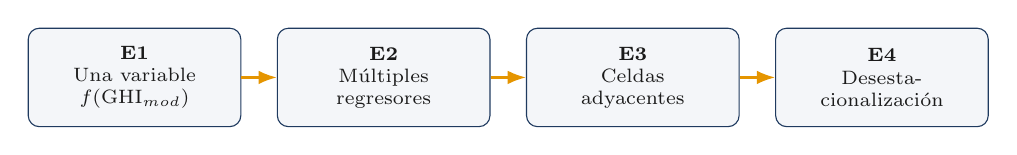
\begin{tikzpicture}[node distance=0.35cm and 0.45cm,
      box/.style={draw=primary,fill=lightbg,rounded corners,minimum width=2.7cm,minimum height=1.25cm,align=center,font=\scriptsize,text=darktext}]
    \node[box] (e1) {\textbf{E1}\\ Una variable\\ $f(\mathrm{GHI}_{mod})$};
    \node[box,right=of e1] (e2) {\textbf{E2}\\ Múltiples\\ regresores};
    \node[box,right=of e2] (e3) {\textbf{E3}\\ Celdas\\ adyacentes};
    \node[box,right=of e3] (e4) {\textbf{E4}\\ Desesta-\\ cionalización};
    \draw[-{Latex},accent,thick] (e1)--(e2);
    \draw[-{Latex},accent,thick] (e2)--(e3);
    \draw[-{Latex},accent,thick] (e3)--(e4);
  \end{tikzpicture}
  \vspace{0.6em}
  \begin{block}{La pregunta que atraviesa el capítulo}
    \footnotesize ¿La mejora viene de la \textbf{complejidad del algoritmo} o de la \textbf{estructura de la información} que le damos?
  \end{block}
\end{frame}

\begin{frame}{Enfoque 1 — Adaptación con una sola variable}
  \footnotesize
  \begin{columns}[T]
    \column{0.5\linewidth}
    \[ \mathrm{GHI}_{adaptada} = f(\mathrm{GHI}_{modelada}) \]
    \begin{itemize}
      \item Corrige el sesgo global; mejora en \textbf{todos} los sitios, pero de forma acotada.
      \item Ejemplo Ero (15 min): RMSE de \textbf{40.9\%} (CAMS) y \textbf{26.5\%} (LSA-SAF) baja a $\sim$31\% y $\sim$25\%.
      \item La mejora es mayor donde el modelo crudo era peor (más margen).
    \end{itemize}
    \column{0.5\linewidth}
    \centering
    \sfig[\linewidth]{scatter_ero_1.png}\\
    {\scriptsize\color{midgray} Ero: los adaptados se acercan a la línea 1:1.}
  \end{columns}
\end{frame}

\begin{frame}[fragile]{Enfoque 1 — Hallazgo clave: SLR $\approx$ MLP $\approx$ XGB}
  \footnotesize
  \begin{columns}[T]
    \column{0.46\linewidth}
    \begin{itemize}
      \item Con \textbf{un único regresor}, lineales y no lineales rinden casi igual.
      \item La calidad del dato de entrada impone un \textbf{techo} a lo que un modelo sofisticado puede ganar.
      \item El MLP puede \emph{sobreajustar} con un solo regresor (menos consistente entre métricas).
    \end{itemize}
    \clave{Aumentar la complejidad del algoritmo, por sí solo, no compra precisión.}
    \column{0.54\linewidth}
    \centering
    % Gráfico nativo con datos reales (rRMSE 15 min, CAMS)
    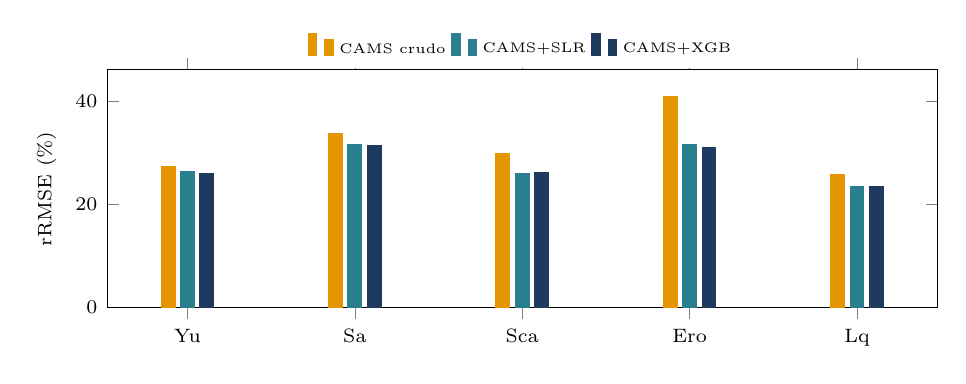
\begin{tikzpicture}
    \begin{axis}[
        width=\linewidth,height=4.6cm,
        ybar,bar width=5pt,
        ymin=0,ymax=46,
        ylabel={\scriptsize rRMSE (\%)},
        symbolic x coords={Yu,Sa,Sca,Ero,Lq},
        xtick=data,
        tick label style={font=\scriptsize},
        ylabel style={font=\scriptsize},
        legend style={font=\tiny,at={(0.5,1.18)},anchor=north,legend columns=3,draw=none},
        enlarge x limits=0.12,
        nodes near coords style={font=\tiny,rotate=90,anchor=west}]
      \addplot[fill=accent,draw=accent] coordinates {(Yu,27.2)(Sa,33.7)(Sca,29.8)(Ero,40.9)(Lq,25.8)};
      \addplot[fill=teal,draw=teal] coordinates {(Yu,26.4)(Sa,31.5)(Sca,26.0)(Ero,31.5)(Lq,23.5)};
      \addplot[fill=primary,draw=primary] coordinates {(Yu,26.0)(Sa,31.4)(Sca,26.2)(Ero,30.9)(Lq,23.5)};
      \legend{CAMS crudo, CAMS+SLR, CAMS+XGB}
    \end{axis}
    \end{tikzpicture}\\
    {\scriptsize\color{midgray} CAMS, 15 min: crudo vs adaptado (datos de la tesis).}
  \end{columns}
\end{frame}

\begin{frame}{Enfoque 2 — Múltiples regresores: primero, análisis exploratorio}
  \footnotesize
  Se parte de un conjunto amplio de variables astronómicas, atmosféricas y meteorológicas (N, SZA, $\alpha$, TOA, GHIargp2, $\delta$, Fn, E0, mr, tm, viento, vapor de agua, punto de rocío) y se \textbf{selecciona} por relevancia física y estadística.
  \vspace{0.4em}
  \begin{block}{Correlación de Pearson/Spearman con la GHI medida}
    \scriptsize
    \begin{itemize}
      \item \textbf{GHIargp2} (cielo claro): 0.71–0.87 — la más informativa.
      \item \textbf{tm} (temperatura media ERA5): 0.41–0.55 — moderada y coherente.
      \item Humedad (tcwv, d2m): correlación muy baja $\Rightarrow$ se descartan.
    \end{itemize}
  \end{block}
  \clave{Seleccionar variables relevantes pesa más que sumar regresores: reduce multicolinealidad y sobreajuste.}
\end{frame}

\begin{frame}{Enfoque 2 — Lo que el filtro de correlación sí y no captura}
  \footnotesize
  \begin{columns}[T]
    \column{0.5\linewidth}
    \textbf{Redundancia exacta: SZA y $\alpha$}
    \begin{itemize}
      \item $\alpha = 90^\circ - \mathrm{SZA}$: información idéntica.
      \item Correlación lineal perfecta $\Rightarrow$ el filtro de Pearson \textbf{la detecta y elimina una} antes de entrenar.
    \end{itemize}
    \column{0.5\linewidth}
    \textbf{Redundancia oculta: N y $\delta$}
    \begin{itemize}
      \item $\delta$ es función determinística de N, pero \textbf{periódica y no monótona}.
      \item Pearson \emph{y} Spearman quedan bajos $\Rightarrow$ el filtro \textbf{no} la captura; ambas se conservan.
      \item Inocuo: N y $\delta$ tienen correlación débil con la GHI $\Rightarrow$ contribución marginal.
    \end{itemize}
  \end{columns}
  \vspace{0.3em}
  \clave{Es una decisión consciente, no un error: el filtro lineal resuelve la colinealidad lineal, no la dependencia no lineal. Mejora menor a futuro: RFE/LASSO o selección sensible a no linealidades.}
\end{frame}

\begin{frame}{Enfoque 2 — Resultado: GHIargp2 + tm, gran salto}
  \footnotesize
  \begin{columns}[T]
    \column{0.46\linewidth}
    Con sólo $\mathrm{GHI}_{mod}$, GHIargp2 y tm (horaria), el error cae fuerte y de forma \textbf{consistente entre sitios}:
    \begin{itemize}
      \item Ero (CAMS): RMSE $\to$ \textbf{19.6\%}.
      \item Lq (CAMS): RMSE $\to$ \textbf{16.0\%}.
      \item Desaparecen los empeoramientos puntuales del conjunto completo.
    \end{itemize}
    \clave{Selección física $\Rightarrow$ mejor ajuste \emph{y} mejor generalización.}
    \column{0.54\linewidth}
    \centering
    \sfig[\linewidth]{rmsd_filtrados.png}\\
    {\scriptsize\color{midgray} Crudo vs adaptado (MLR/MLP/XGB) con regresores seleccionados.}
  \end{columns}
\end{frame}

\begin{frame}{Enfoque 3 — Celdas satelitales adyacentes}
  \footnotesize
  \begin{columns}[T]
    \column{0.5\linewidth}
    \begin{itemize}
      \item La irradiancia de un sitio forma parte de un campo \textbf{espacialmente coherente} (sistemas nubosos de mesoescala, decenas de km).
      \item Se incorporan como regresores las celdas vecinas (vecindad de von Neumann, \textbf{DM=1}: cuatro celdas cardinales).
      \item Rompe el paradigma clásico de \textbf{una sola celda}.
    \end{itemize}
    \clave{Aporta contexto espacial que un modelo de celda única no puede ver.}
    \column{0.5\linewidth}
    \centering
    \sfig[\linewidth]{analogiaVecinos.png}\\
    {\scriptsize\color{midgray} Analogía espacial: celdas y dinámica atmosférica.}
  \end{columns}
\end{frame}

\begin{frame}{Enfoque 3 — Resultado: el contexto espacial manda, no el algoritmo}
  \footnotesize
  \begin{columns}[T]
    \column{0.5\linewidth}
    \begin{itemize}
      \item Reducciones de RMSE del orden de \textbf{5–15\%} según sitio y producto.
      \item Mayor mejora en entornos de alta variabilidad topográfica/atmosférica.
      \item \textbf{MLR estable} frente a MLP/XGB: la ganancia viene de la \emph{información}, no de la complejidad.
      \item Sumar temperatura (caso TM2) refuerza la corrección.
      \item Robusto a 15 min y horario.
    \end{itemize}
    \column{0.5\linewidth}
    \centering
    \sfig[\linewidth]{rmsd_vecinos.png}\\
    {\scriptsize\color{midgray} rRMSE con el enfoque de celdas adyacentes.}
  \end{columns}
\end{frame}

\begin{frame}{Enfoque 4 — Desestacionalización}
  \footnotesize
  Tres formulaciones sobre regresión lineal:
  \begin{itemize}
    \item \textbf{E1} directo: $\mathrm{GHI}_{ad}=a\,\mathrm{GHI}_{mod}+b$.
    \item \textbf{E2} (Salamalikis): modela el error $\Delta_{\mathrm{GHI}}=\mathrm{GHI}_{med}-\mathrm{GHI}_{mod}$.
    \item \textbf{E3} desestacionaliza con cielo claro (ARGP-V2): $X=\mathrm{GHI}_{mod}-\mathrm{GHI}_{cc}$, $Y=\mathrm{GHI}_{med}-\mathrm{GHI}_{cc}$.
  \end{itemize}
  \vspace{0.3em}
  \begin{block}{Resultado conceptual}
    \scriptsize E1 y E2 son \textbf{matemáticamente equivalentes} bajo regresión lineal. E3 aísla la componente determinística (geometría solar) y deja que la regresión aprenda sólo la \textbf{variabilidad atmosférica residual}: más estable y \textbf{interpretable} ($a$, $b$ con sentido físico).
  \end{block}
  \clave{Especialmente valioso donde la estructura estacional es fuerte (Ero, Lq).}
\end{frame}

\begin{frame}[fragile]{Síntesis comparativa — la conclusión matizada}
  \scriptsize
  \begin{columns}[T]
    \column{0.5\linewidth}
    LSA-SAF horario, dos extremos: \textbf{Sa} (valle, peor caso) y \textbf{Ero} (altiplano, mejor caso).
    \vspace{0.3em}
    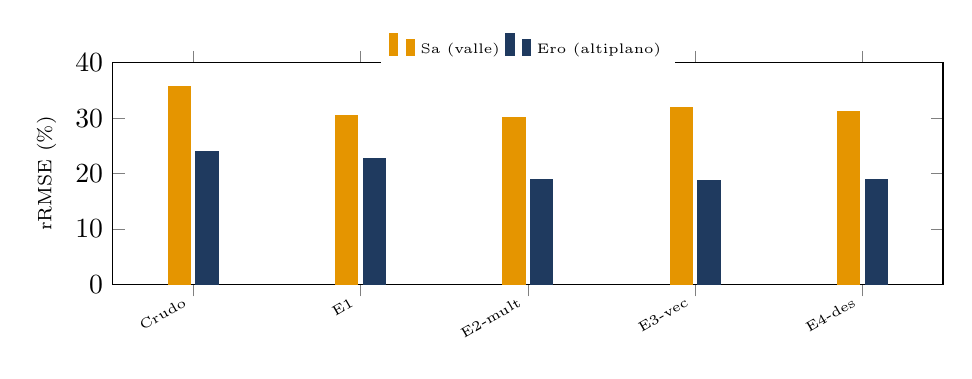
\begin{tikzpicture}
    \begin{axis}[
        width=\linewidth,height=4.4cm,
        ybar,bar width=8pt,ymin=0,ymax=40,
        ylabel={\scriptsize rRMSE (\%)},
        symbolic x coords={Crudo,E1,E2-mult,E3-vec,E4-des},
        xtick=data,
        x tick label style={font=\tiny,rotate=30,anchor=east},
        ylabel style={font=\scriptsize},
        legend style={font=\tiny,at={(0.5,1.16)},anchor=north,legend columns=2,draw=none},
        enlarge x limits=0.12]
      \addplot[fill=accent,draw=accent] coordinates {(Crudo,35.7)(E1,30.5)(E2-mult,30.1)(E3-vec,31.9)(E4-des,31.1)};
      \addplot[fill=primary,draw=primary] coordinates {(Crudo,24.0)(E1,22.8)(E2-mult,18.9)(E3-vec,18.8)(E4-des,18.9)};
      \legend{Sa (valle), Ero (altiplano)}
    \end{axis}
    \end{tikzpicture}
    \column{0.5\linewidth}
    \begin{itemize}
      \item \textbf{El sesgo siempre se corrige}: en Sa, MBE 17.9\%$\to\sim$4\%; en Ero, $-7.7\%\to\sim$+1\%.
      \item Dentro de un enfoque, \textbf{el regresor casi no cambia el resultado}.
      \item En \textbf{Ero} (cielo claro, fuerte estacionalidad), E2/E3/E4 convergen y mejoran mucho sobre E1.
      \item En \textbf{Sa} (valle convectivo) hay un \textbf{piso estructural} ($\sim$30–32\%): ni el espacio ni la desestacionalización lo superan.
    \end{itemize}
  \end{columns}
\end{frame}

\begin{frame}{El mensaje central de los resultados}
  \footnotesize
  \begin{block}{Estructura de la información $>$ complejidad del algoritmo}
    El factor determinante de la mejora es \textbf{qué información se incorpora} —variables físicamente relevantes, contexto espacial, remoción de estacionalidad— y no el algoritmo de regresión. Un MLR bien alimentado iguala a MLP/XGB con menor costo y mayor interpretabilidad.
  \end{block}
  \begin{block}{Recomendación operativa matizada}
    \scriptsize
    \begin{itemize}
      \item Error dominado por \textbf{sesgo + estacionalidad} (altura, cielo claro) $\Rightarrow$ E2/E3/E4 son intercambiables; elegir por costo/interpretabilidad.
      \item Error dominado por \textbf{procesos locales de alta frecuencia} (valle convectivo) $\Rightarrow$ la SA quita el sesgo pero choca con un piso; la mejora futura depende de \emph{productos de mayor resolución}, no de más adaptación.
    \end{itemize}
  \end{block}
\end{frame}

%==================================================================
\section{Generalización espacial}
%==================================================================

\begin{frame}{El problema que queda: la corrección es local}
  \footnotesize
  \begin{itemize}
    \item Cada modelo se ajusta donde \emph{hay} medición. ¿Cómo llevarlo a celdas sin medición?
    \item Primero hay que saber \textbf{cuán lejos} puede viajar un modelo ajustado.
  \end{itemize}
  \vspace{0.3em}
  \clave{Sin una regla de transferencia, la SA se queda en los pocos puntos instrumentados — justo lo que se quería superar.}
\end{frame}

\begin{frame}{Validación cruzada entre sitios: transferencia direccional}
  \footnotesize
  \begin{columns}[T]
    \column{0.5\linewidth}
    \begin{itemize}
      \item Entrenar en un sitio, probar en otro (modelo ERA5, MLR).
      \item El error crece cuando difieren las condiciones ambientales.
      \item Modelos de \textbf{alta montaña} transfieren bien a otra alta montaña; de baja altitud, a baja altitud.
      \item Transferencia \textbf{asimétrica}: A$\to$B no implica B$\to$A.
      \item La \textbf{altitud} emerge como variable de control (estructura térmica, humedad).
    \end{itemize}
    \column{0.5\linewidth}
    \centering
    \sfig[\linewidth]{deltaCrossValidationOneSite.png}\\
    {\scriptsize\color{midgray} $\Delta$rRMSE: filas=entrenamiento, columnas=prueba.}
  \end{columns}
\end{frame}

\begin{frame}{Propuesta: asignación por distancia 3D (lat, lon, altitud)}
  \footnotesize
  \begin{columns}[T]
    \column{0.5\linewidth}
    A cada celda sin medición se le asigna el modelo de la estación \textbf{más cercana en 3D}:
    \[ D_i=\sqrt{(x'-x_i')^2+(y'-y_i')^2+(z'-z_i')^2} \]
    \begin{itemize}
      \item Coordenadas normalizadas (\emph{z-score}) para que la altitud pese igual que lat/lon.
      \item Búsqueda eficiente con \textbf{KD-Tree}.
      \item Garantiza continuidad espacial del campo corregido, escalable a todo el dominio.
    \end{itemize}
    \column{0.5\linewidth}
    \centering
    \sfig[\linewidth]{distancia3d.png}\\
    {\scriptsize\color{midgray} El punto objetivo (verde) hereda el modelo de la estación más próxima.}
  \end{columns}
\end{frame}

\begin{frame}{Validación independiente: Abra Pampa y Cerrillos (ERA5)}
  \scriptsize
  \begin{columns}[T]
    \column{0.5\linewidth}
    Dos estaciones \textbf{no} usadas en el ajuste (ex-red ENARSOL, 2017). El criterio 3D asigna: Ap$\to$modelo de Lq; Ce$\to$modelo de Sa.
    \vspace{0.4em}
    \renewcommand{\arraystretch}{1.2}
    \begin{tabular}{@{}lcc@{}}
      \toprule
       & \textbf{Ap} RMSE & \textbf{Ce} RMSE\\
      \midrule
      ERA5 crudo    & 19.7\% & 38.1\%\\
      ERA5 ajustado & 19.6\% & 36.5\%\\
      \midrule
       & \textbf{Ap} MBE & \textbf{Ce} MBE\\
      \midrule
      ERA5 crudo    & 2.6\% & 13.4\%\\
      ERA5 ajustado & 1.8\% & \textbf{7.8\%}\\
      \bottomrule
    \end{tabular}
    \column{0.5\linewidth}
    \begin{itemize}
      \item \textbf{Cerrillos}: sesgo reducido \textbf{más del 40\%}.
      \item \textbf{Abra Pampa}: casi sin cambio — ERA5 ya representa bien la alta montaña seca; aun así baja el MBE.
      \item Mejoras modestas pero \textbf{consistentes}, y un campo regional espacialmente coherente.
    \end{itemize}
    \clave{La transferencia por similitud geográfica-altitudinal funciona en sitios nunca vistos.}
  \end{columns}
\end{frame}

\begin{frame}{¿Por qué ERA5 para la generalización?}
  \footnotesize
  \begin{itemize}
    \item La generalización exige, en \emph{cada} celda sin medición, tanto la GHI como \textbf{todos los regresores} usados en la adaptación.
    \item ERA5 provee irradiancia y covariables meteorológicas sobre \textbf{una misma grilla global, regular y continua}.
    \item LSA-SAF es más preciso puntualmente, pero \textbf{no} ofrece el conjunto completo de regresores de forma auto-consistente en puntos arbitrarios.
  \end{itemize}
  \vspace{0.3em}
  \clave{El criterio de generalización es independiente del producto; extenderlo a productos satelitales es trabajo futuro.}
\end{frame}

%==================================================================
\section{Conclusiones y perspectivas}
%==================================================================

\begin{frame}{Conclusiones (1/2)}
  \footnotesize
  \begin{block}{Sobre los modelos crudos}
    \scriptsize Satélite $>$ reanálisis en general, pero insuficientes para alta precisión en el NOA sin ajuste local; la fiabilidad no es uniforme (CAMS/Ero).
  \end{block}
  \begin{block}{Sobre la adaptación con regresores}
    \scriptsize Mejora en todos los sitios. \textbf{MLR bien configurado} basta en la mayoría de los casos; MLP/XGB se justifican sólo con más regresores y no linealidades marcadas. El \textbf{contexto espacial} (celdas adyacentes) es uno de los mayores aportes.
  \end{block}
  \begin{block}{Sobre generalización}
    \scriptsize Los modelos adaptados conservan desempeño si hay \textbf{similitud geográfica y altitudinal}; habilita mapas regionales más confiables que los puramente satelitales.
  \end{block}
\end{frame}

\begin{frame}{Conclusiones (2/2) — Aportes de la tesis}
  \footnotesize
  \begin{enumerate}
    \item Diagnóstico detallado del desempeño de modelos de GHI actuales en el NOA (15 min y horario).
    \item Metodología de \textbf{Adaptación al Sitio con múltiples regresores}, propuesta y validada.
    \item Demostración del valor de la \textbf{información espacialmente coherente} (celdas adyacentes).
    \item Confirmación de que la SA puede \textbf{generalizarse} para construir mapas regionales de mejor calidad.
  \end{enumerate}
  \vspace{0.4em}
  \clave{Metodología reproducible, escalable y de bajo costo: una alternativa eficaz frente a expandir redes de medición costosas.}
\end{frame}

\begin{frame}{Producción científica asociada}
  \scriptsize
  \textbf{Artículos en revistas con arbitraje}
  \begin{itemize}
    \item \emph{Machine Learning for Site Adaptation of Satellite-Derived Solar Irradiance in NW Argentina.} Ledesma \& Salazar. \textbf{J. of Computer Science \& Technology}, 25(2), 2025.
    \item \emph{Machine Learning Site Adaptation for Optimizing Heliosat-4 GHI using Adjacent Satellite Cells.} Ledesma, Salazar, López, Nollas. \textbf{ASME J. Solar Energy Eng.}, 2026.
    \item \emph{Performance Evaluation of Solar Irradiance Models at 11 Sites in South America.} Ledesma \& Salazar. \textbf{ASME J. Solar Energy Eng.} (aceptado).
  \end{itemize}
  \textbf{Congreso con arbitraje}
  \begin{itemize}
    \item \emph{Site Adaptation for GHI in Argentina Using a Multilayer Perceptron.} Salazar, Gueymard, Ledesma, Vilela. \textbf{ISES Solar World Congress 2025}, Fortaleza.
  \end{itemize}
\end{frame}

\begin{frame}{Perspectivas a futuro}
  \footnotesize
  \begin{itemize}
    \item \textbf{Nuevas fuentes}: GOES-16/19 (mejor posicionamiento sobre el NOA).
    \item \textbf{Vecindad espacio-temporal}: añadir información diferenciada en el tiempo, no sólo vecinos simultáneos.
    \item \textbf{Producción FV real}: validar y ajustar desde la energía, no sólo radiométricamente.
    \item \textbf{Expandir la validación cruzada}: nuevas estaciones de alta montaña.
    \item \textbf{Herramientas operativas}: plataformas web / API para instituciones.
    \item \textbf{Selección automática} (RFE, LASSO, permutación) y desestacionalización avanzada (Fourier, STL, wavelets).
  \end{itemize}
\end{frame}

\begin{frame}[plain]
  \begin{tikzpicture}[remember picture,overlay]
    \fill[primary] (current page.south west) rectangle (current page.north east);
    \fill[accent] ([yshift=2.1cm]current page.center -| current page.west) rectangle ([yshift=2.2cm]current page.center -| current page.east);
  \end{tikzpicture}
  \vfill\centering
  {\color{white}\Large\bfseries Gracias.}\\[0.6em]
  {\color{white}\footnotesize Quedo a disposición del jurado para las preguntas.}\\[0.01em]
  {\color{white!80}\scriptsize Rubén D. Ledesma}
  \vfill
\end{frame}

%==================================================================
%  ANEXO / RESPALDO PARA PREGUNTAS  (no contar en los 55 min)
%==================================================================
\begin{frame}[plain]
  \centering\vfill
  {\color{primary}\Large\bfseries Diapositivas de respaldo}\\[0.4em]
  {\color{midgray}\footnotesize Material de apoyo para el turno de preguntas}
  \vfill
\end{frame}

\begin{frame}{Respaldo — ¿Un año de overlap es suficiente \emph{y} hay riesgo de estacionariedad?}
  \footnotesize
  \begin{block}{La tensión aparente}
    \scriptsize Sostengo que $\sim$1 año de overlap basta para \emph{entrenar}, y a la vez listo la no estacionariedad como limitación. ¿Contradicción?
  \end{block}
  \textbf{Respuesta:} son dos afirmaciones sobre planos distintos.
  \begin{itemize}
    \item \textbf{Suficiencia estadística} (entrenamiento): un año cubre el ciclo estacional completo $\Rightarrow$ alcanza para \emph{estimar} $a$, $b$ y capturar la relación.
    \item \textbf{Validez de la extrapolación} (aplicación): aplicar esa función a \emph{décadas} supone que la relación no deriva. Eso depende de la \textbf{representatividad} del año elegido y de la estabilidad del producto, no de la cantidad de datos.
  \end{itemize}
  \clave{Un año basta para \emph{ajustar}; la estacionariedad gobierna por cuánto tiempo ese ajuste sigue siendo válido. No compiten.}
\end{frame}

\begin{frame}{Respaldo — Incertidumbre instrumental y el piso de error}
  \scriptsize
  \begin{itemize}
    \item Fuentes: calibración y su deriva, respuesta direccional/coseno, dependencia térmica, no linealidad, selectividad espectral, \emph{thermal offset} (termopila).
    \item CMP11/PSP (clase A) vs CMP3 (clase inferior): \textbf{pisos de incertidumbre desiguales} entre sitios.
    \item La GHI medida es la referencia de las tres métricas $\Rightarrow$ su error se propaga y fija un mínimo.
    \item \textbf{Lectura honesta}: mejoras del orden de la incertidumbre de medición no son, por sí solas, prueba concluyente de mejora del modelo. Las conclusiones se apoyan en las diferencias que \emph{superan} ese margen.
    \item Mitigación: calibración periódica trazable en GERSolar (UNLu).
  \end{itemize}
\end{frame}

\begin{frame}{Respaldo — ¿Por qué vecindad DM=1 y no DM=2?}
  \footnotesize
  \begin{itemize}
    \item Se adoptó la vecindad de \textbf{von Neumann (DM=1)}: las cuatro celdas cardinales, no las ocho de Moore.
    \item \textbf{Decisión de diseño}, no omisión: prioriza coherencia espacial de primer orden con un número acotado de regresores (menos multicolinealidad y sobreajuste).
    \item En la síntesis comparativa, las celdas adyacentes ya igualan o superan a múltiples regresores en altura, sin necesidad de ampliar el vecindario.
    \item \textbf{Limitación reconocida}: DM=2 (o vecindades ponderadas por distancia) podría capturar estructuras nubosas mayores — línea de trabajo futura.
  \end{itemize}
\end{frame}

\begin{frame}{Respaldo — Definiciones de índices}
  \scriptsize
  \begin{itemize}
    \item \textbf{$k_t$} (índice de claridad): GHI / irradiancia teórica en el tope de la atmósfera sobre plano horizontal.
    \item \textbf{Índice de variabilidad}: desviación estándar de las diferencias consecutivas de GHI en una ventana ($N=10$):
      \[ \mathrm{VarIndex}(t)=\sqrt{\tfrac{1}{N-1}\textstyle\sum_{i\in\mathcal{W}(t)}\big[(\mathrm{GHI}_i-\mathrm{GHI}_{i-1})-\overline{\Delta\mathrm{GHI}}\big]^2} \]
    \item \textbf{SZA / $\alpha$}: ángulo cenital solar y altura solar, $\alpha=90^\circ-\mathrm{SZA}$.
    \item \textbf{GHIargp2}: GHI de cielo despejado (modelo ARGP-V2, Ledesma 2023a).
    \item \textbf{E0}: factor de corrección Tierra–Sol; \textbf{mr}: masa de aire relativa.
  \end{itemize}
\end{frame}

\begin{frame}{Respaldo — Medias de GHI por sitio (normalización de métricas)}
  \scriptsize
  \centering
  \renewcommand{\arraystretch}{1.3}
  \begin{tabular}{@{}lccccc@{}}
    \toprule
    Sitio & Yu & Sa & Sca & Ero & Lq\\
    \midrule
    GHI media (W/m²) & 429.2 & 432.9 & 554.4 & 628.4 & 648.7\\
    \bottomrule
  \end{tabular}
  \vspace{0.8em}
  \par Todas las métricas relativas (\%) de la tesis están normalizadas respecto a estos valores, lo que permite comparar de forma justa sitios de valle y de altiplano.
\end{frame}

\end{document}
